\documentclass[journal,onecolumn]{IEEEtran}

\title{Applied Spatial and Temporal Data Analysis}
\author{Vijay K. Shah}

\usepackage{amsmath}
\usepackage{mathtools}
\usepackage{graphicx}
\usepackage{enumitem}
\usepackage{epsfig}
\usepackage{color}
\usepackage{algorithm}
\usepackage[noend]{algpseudocode}
\usepackage{subfigure}
\usepackage[justification=centering]{caption}
\usepackage{csvsimple}
\usepackage{longtable}

\begin{document}
\maketitle

\section{Preliminary Details}
For this assignment, I have created three different folders, namely \\
\begin{enumerate}
\item \textbf{PythonFiles:} This folder contains all the python files. \\
\item \textbf{OutputFiles:} This folder contains all the output files corresponding to each python file. For example, for python file $svd.py$ (in folder \textit{PythonFiles}, I have saved its output in  a file named $svd.txt$ in this folder. \\
\item \textbf{images:} This folder contains all the plots that have been shown in this report. \\
\end{enumerate}

Besides these, I have a file named \textit{recommendation$\_$command.txt} which basically contains all the \textbf{GNUPLOT} scripts to generate the plots. To run this file, you may simple run $<$\textbf{gnuplot recommendation$\_$command.txt} $>$in terminal and all the plots would be generated in folder \textbf{images}.


\section{Comparative Performance Analysis}

\textit{Q 9. Compare the performances of User-based collaborative filtering, item-based collaborative filtering, SVD, PMF, NMF on fold-1 with respect to RMSE and MAE. Since data.split(n-folds=3) randomly split the data into 3 folds, please make sure you test the five algorithms on the same fold-1 so the results are comparable.} 

\textit{Q 10. Compare the performances of User-based collaborative filtering, item-based collaborative
filtering, SVD, PMF, NMF on fold-2 with respect to RMSE and MAE. Please make sure you test
the five algorithms on the same fold-2 so the results are comparable. }

\textit{Q 11. Compare the performances of User-based collaborative filtering, item-based collaborative
filtering, SVD, PMF, NMF on fold-3 with respect to RMSE and MAE. Please make sure you test
the five algorithms on the same fold-3 so the results are comparable. }

\textit{Q 12: Compare the average (mean) performances of User-based collaborative filtering, item-based
collaborative filtering, SVD, PMF, NMF with respect to RMSE and MAE. Please make sure you
test the five algorithms on the same 3-fold data split plan so the results are comparable. } \\

 In this section, we first define the two famous metrics (i) MAE and (ii) RMSE for evaluating the performances of a recommender system. Then, we discuss the comparative performance analysis of two classes of recommendation algorithms -- (i) Matrix Factorization (such as SVD, PMF and NMF) and (ii) Collaborative Filtering (such as UCF and ICF).

\subsection{Definitions}
\begin{itemize}
\item \textbf{Mean Absolute Error (MAE)} measures how close the predictions are to the true (actual) values. MAE is calculated as follows:
\begin{equation}
MAE = \frac{1}{n} \sum_{i=1}^n |f_i - y_i|
\end{equation}

where $n$ is the total number of observations, $f_i$ is the prediction and $y_i$ is the true value.

\item \textbf{Root Mean Square Deviation (RMSD)} measures the differences between the predicted values by a model and the values actually observed. RMSD is calculated as follows:
\begin{equation}
RMSD = \sqrt{\frac{1}{n} \sum_{i=1}^{n} (f_i - y_i)^2}
\end{equation}
where $n$ is the total number of observations, $f_i$ is the predicted value and $y_i$ is the actual value.
\end{itemize}

\subsection{Fold-wise Performance Analysis for Different Recommendation Algorithms}
As shown in Fig. \ref{fold1} (Fold 1), Fig. \ref{fold2} (Fold 2), Fig.  \ref{fold3} (Fold 3) and Fig. \ref{mean} (Average), for both RMSE and MAE, matrix factorization recommendation algorithms viz. SVD, PMF and NMF perform better than collaborative filtering ones i.e. UCF and ICF. In particular, SVD yields least error whereas User (UCF) and Item-based collaborative filtering (ICF) perform the worst. This is because SVD uses the k-largest singular values of matrix A (where the rows are users, columns are items and value of each cell is the rating) to construct a matrix $A_k$ to approximate A. Whereas, UCF simply estimates each user's preferences by referring to his/her similar user's tastes and ICF recommends items which are similar to the target user's selected items. These two collaborative filtering approaches are prone to noise and local optimal recommendations, hence yield higher error than the SVD constructs a provably-best k-rank approximation, and hence does generalized globally optimized recommendations.

\begin{figure}[H]
\begin{center}
 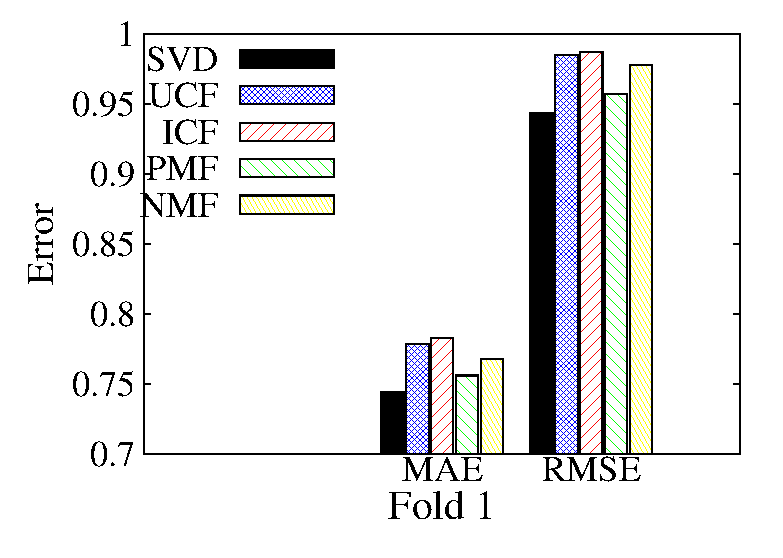
\includegraphics[scale = 0.98] {images/fold1.eps}
 \caption {Fold 1 - Error against different algorithms} \label{fold1}
 \end{center}
\end{figure}


\begin{figure}[H]
\begin{center}
 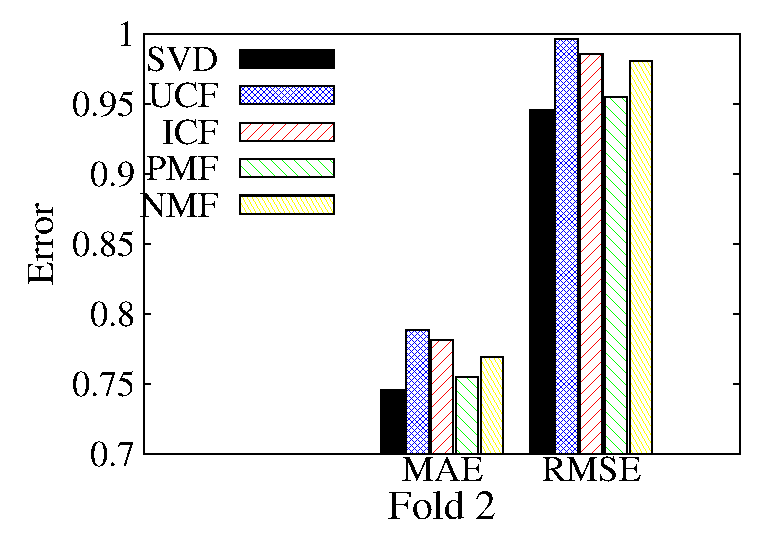
\includegraphics[scale = 0.98] {images/fold2.eps}
 \caption {Fold 2 - Error against different algorithms} \label{fold2}
 \end{center}
\end{figure}

\begin{figure}[H]
\begin{center}
 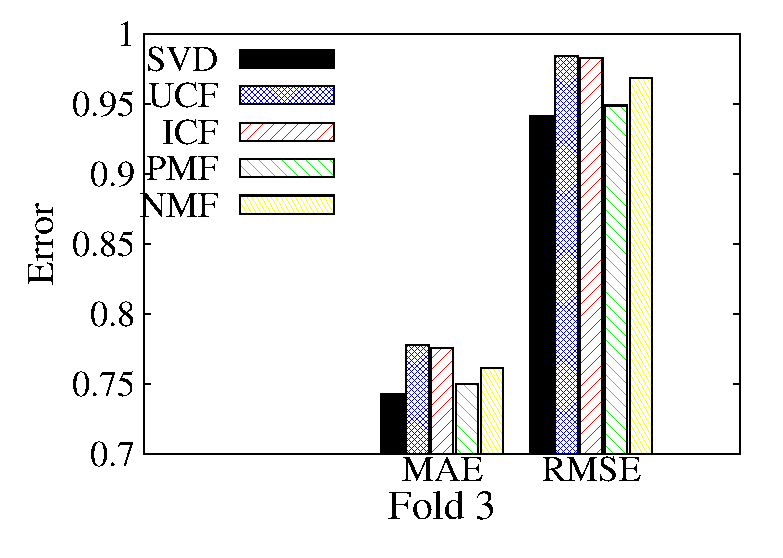
\includegraphics[scale = 0.98] {images/fold3.eps}
 \caption {Fold 3 - Error against different algorithms} \label{fold3}
 \end{center}
\end{figure}


\begin{figure}[H]
\begin{center}
 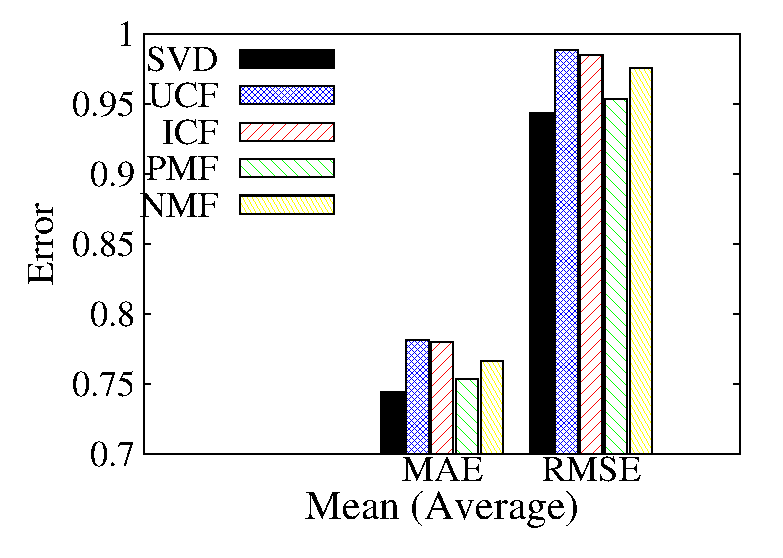
\includegraphics[scale = 0.98] {images/mean.eps}
 \caption {Average - Error against different algorithms} \label{mean}
 \end{center}
\end{figure}

\textit{Q 13: Examine how the cosine, MSD (Mean Squared Difference), and Pearson similarities impact the
performances of User based Collaborative Filtering and Item based Collaborative Filtering. Finally, is the impact of the three metrics on User based Collaborative Filtering consistent with the impact of the three metrics on Item based Collaborative Filtering? Plot your results.} \\

In this section, we first formally introduce cosine, MSD and Pearson similarity metrics followed by detailed analysis of these similarity metrics on the performances of UCF and ICF.

\subsection{Definitions}
\begin{itemize}
\item \textbf{Cosine}: The cosine similarity is defined as follows:
\begin{equation}
cosine-sim(u, v) = \frac{\sum_{i =1}^{m} r_{ui} r_{vi}}{\sqrt{\sum_{i =1}^{m} r_{ui}^2} \sqrt{\sum_{i =1}^{m} r_{vi}^2}}
\end{equation}

where $u$ and $v$ are two users (or items) and $m$ is the total number of users (or items). It is important to note that only common users (or items) are taken into account.

\item \textbf{Mean Squared Difference (MSD)} The Mean Squared Difference is defined as:
\begin{equation}
msd(u, v) = \frac{1}{m} \sum_{i=1}^m (r_{ui} - r_{vi})^2
\end{equation}
where $u$ and $v$ are two users (or items) and $m$ is the total number of users (or items). It is important to note that only common users (or items) are taken into account.

\item \textbf{Pearson correlation coefficient}: The Pearson correlation coefficient is defined as:
\begin{equation}
pearson-sim(u,v) = \frac{\sum_{i=1}^m (r_{ui} - \mu_i).(r_{vi} - \mu_{i})}{\sqrt{\sum_{i=1}^m (r_{ui} - \mu_{i})^2} \sqrt{\sum_{j=1}^m (r_{uj} - \mu_{j})^2}}
\end{equation}
where $\mu_{i} = \frac{1}{m} \sum_{i=1}^{m} r_{ui}$ is the sample mean value and analogously for $\mu_{j}$.
\end{itemize}

\subsection{Performance Similarity Metrics Analysis}
As shown in Fig. \ref{mae} and \ref{rmse}, the UCF and ICF are consistent in terms of Mean Squared Difference (MSD). Whereas, in case of Cosine and Pearson, ICF suffers a significantly higher error value (both MAE and RMSE) compared to that of UCF.

\begin{figure}[H]
\begin{center}
\label{thr}
\subfigure[\label{mae}]{
\epsfig{figure=images/mae.eps,width=3.40in,keepaspectratio}}
\subfigure[\label{rmse}]{
\epsfig{figure=images/rmse.eps,width=3.40in,keepaspectratio}}

\caption{UCF vs ICF (a. MAE b. RMSE) }
\end{center}
\end{figure}

\iffalse
\begin{figure}[H]
\begin{center}
 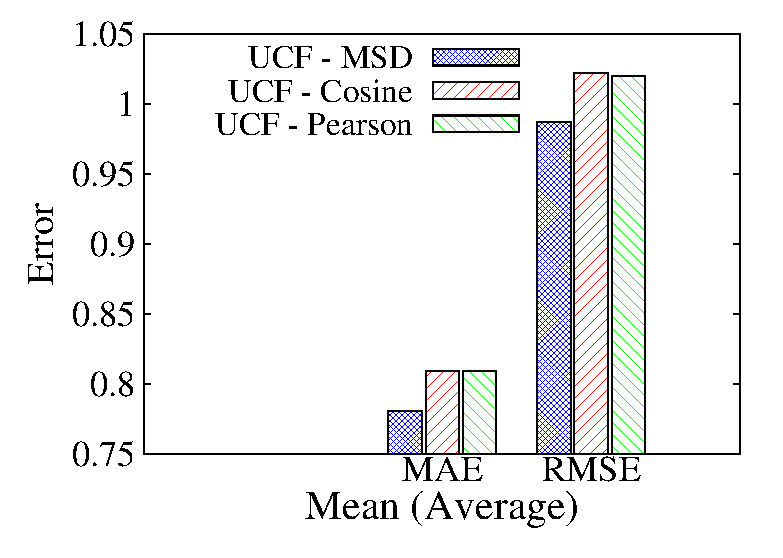
\includegraphics[scale = 0.98] {images/ucfSimilarity.eps}
 \caption { UCF: Analysis of different similarity metrics} \label{ucfSimilarity}
 \end{center}
\end{figure}


\begin{figure}[H]
\begin{center}
 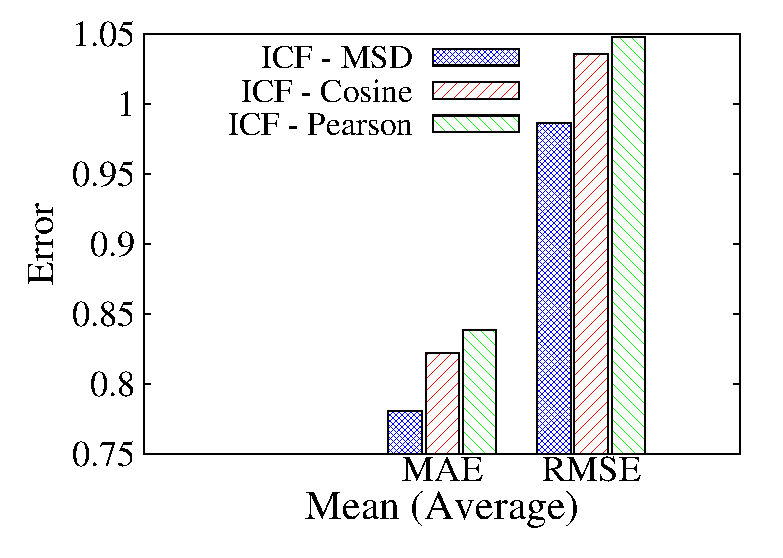
\includegraphics[scale = 0.98] {images/icfSimilarity.eps}
 \caption { ICF: Analysis of different similarity metrics} \label{icfSimilarity}
 \end{center}
\end{figure}
\fi

\textit{Q 14: Examine how the number of neighbors impacts the performances of User based Collaborative
Filtering or Item based Collaborative Filtering? Plot your results.} \\

As shown in Fig. \ref{ucf_1} (for MAE) and \ref{ucf_2} (for RMSE), with increase in $K$ (number of neighbors) the error value for UCF recommendation algorithm first decreases until $K=30$. Also refer Fig. \ref{ucf_3}. However, after that, the error value increases. Hence, the best $K$ is $30$ for the given data set. 

In case of ICF recommendation algorithm also, the error value first  decreases until $K=30$, then, it again start peaking up as shown Fig. \ref{icf_1} (for MAE) and \ref{icf_2} (for RMSE) and \ref{icf_3}. Here, also, the best $K$ is $30$. 

\begin{figure}[H]
\begin{center}
\label{thr}
\subfigure[\label{ucf_1}]{
\epsfig{figure=images/ucfBestK_histo_mae.eps,width=3.40in,keepaspectratio}}
\subfigure[\label{ucf_2}]{
\epsfig{figure=images/ucfBestK_histo_rmse.eps,width=3.40in,keepaspectratio}}

\caption{UCF: a. Error (MAE) vs K b. Error (RMSE ) vs K }
\end{center}
\end{figure}


\begin{figure}[H]
\begin{center}
 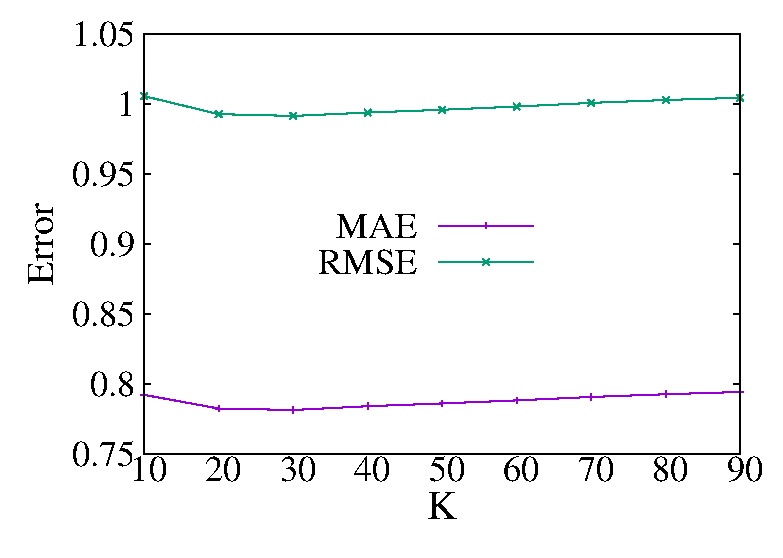
\includegraphics[scale = 0.98] {images/ucfBestK.eps}
 \caption { UCF: Error vs K} \label{ucf_3}
 \end{center}
\end{figure}



\begin{figure}[h]
\begin{center}
\label{thr}
\subfigure[\label{icf_1}]{
\epsfig{figure=images/icfBestK_histo_mae.eps,width=3.40in,keepaspectratio}}
\subfigure[\label{icf_2}]{
\epsfig{figure=images/icfBestK_histo_rmse.eps,width=3.40in,keepaspectratio}}
%\subfigure[\label{icf_3}]{
%\epsfig{figure=icfBestK.eps,width=3.40in,keepaspectratio}}
\caption{ICF: a. Error (MAE) vs K b. Error (RMSE) vs K  }
\end{center}
\end{figure}



\begin{figure}[H]
\begin{center}
 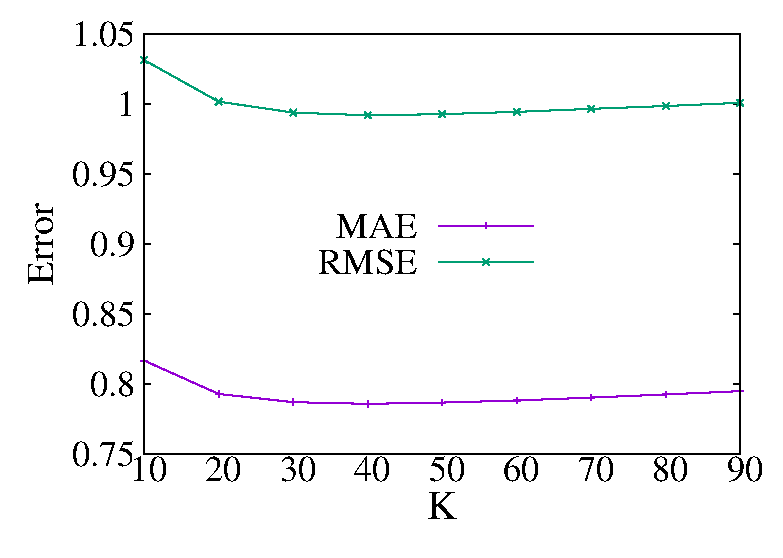
\includegraphics[scale = 0.98] {images/icfBestK.eps}
 \caption {ICF: Error vs  K} \label{icf_3}
 \end{center}
\end{figure}

\section{Conclusion}
From the aforementioned analysis, we can conclude that the matrix factorization recommendation algorithms such as SVD, PMF and NMF predict better than the counterpart Collaborative filtering (CF) algorithms viz. UCF and ICF.  Also, among CF recommendation algorithms, the MSD exhibits lower error value (for both MAE and RMSE) compared to that of Cosine and Pearson similarity metrics. Finally, it is also evident that MAE consistently exhibits low error value compared to that of RMSE irrespective of recommendation algorithms and similarity metrics employed.
\end{document}